In general when using a SLAM the state equation of the robot is known and helps the localization problem, the state equation models the behaviour of the robot in function of input parameters:

\begin{align}
\dot{x} &= v*cos(\theta)\\
\dot{y} &= v*sin(\theta)\\
\dot{\theta} &= u_{1}\\
\dot{v} &= u_{2}
\end{align}

Above is a state equation modelling a car ($x$ and $y$ are the position, $\theta$ is the heading and v the speed), with input $u_{1}$ and $u_{2}$ which are known (the robot computes them).
They are the most used and studied method and many use probability and decision theory to estimate the pose of the robots and the map such as the EKF Slam.

\subsection{EKF SLAM}
An EKF SLAM is a slam algorithm that uses the Extended Kalman filter to accomplish the problem, it is a features based slam.

\subsubsection{Kalman Filter}

The Kalman Filter is used to estimate the linear state equation variable over time keeping track of the uncertainties of the variables, this filter permits data fusion:

\begin{figure}[H]
\centering
    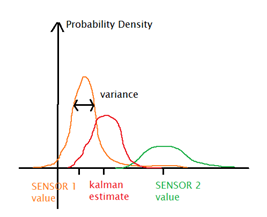
\includegraphics[scale=1]{kalmanExample.png} 
    \caption{Simple example of data fusion.}
    \label{fig:kalexample}
\end{figure}

If we have two sensors that measure the same variable the Kalman filter will combine them in function of their variances (a sensor with great variance means that it is less precise so it is less trustworthy whereas a sensor with little variance will be more precise), in figure~\ref{fig:kalexample} we combine two sensors with a Gaussian noise, this is a simple example of what the Kalman filter can do, it can also combine information between the state variables, (a state variable can be the position, the speed, angular speed ) and if we have relations between those variables (position and speed) the Kalman filter will be able to combine the estimates.\\

Therefore in what way is the Kalman filter used for the slam? The landmarks detected are put in the state equation in order to estimate their position and use them to improve the robot localisation:

\begin{figure}[H]
\centering
    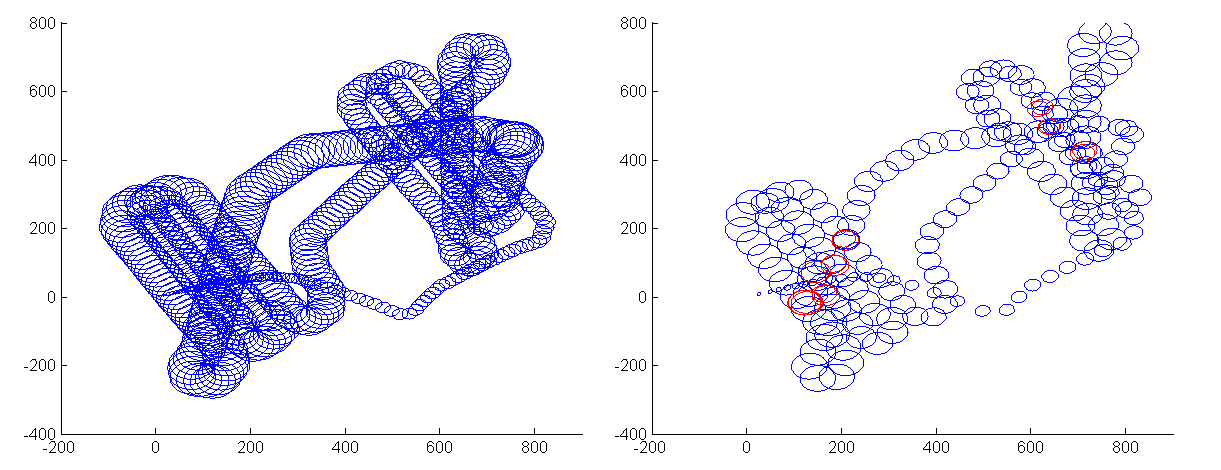
\includegraphics[scale=0.5]{observerKalman.png} 
    \caption{Estimate of position of an underwater vehicle without and with landmarks using a Kalman Filter.}
    \label{fig:obserKalman}
\end{figure}

In figure~\ref{fig:obserKalman} the Kalman filter only uses the model of the underwater vehicle to estimate its position therefore the variance (represented by an ellipse) always increases whereas when landmarks are available it can slow the uncertainty propagation. The extended Kalman filter is used to work on nonlinear problems such as the SLAM problem, thus causing a bit of approximation.

\subsection{FastSLAM}

The FastSLAM algorithm \cite{montemerlo2002fastslam} uses a particle filter and a Kalman filter to solve the SLAM problem, so this is also a landmark based algorithm.\\
The FastSLAM algorithm creates many particles that represent hypothesis on the position of the robot, the particles are randomly placed over the possible position of the robot. Then the landmarks are estimated for each particle using the Extended Kalman filter (supposing the position of the robot known for the particle).\\

After that the likeliness of each particle being the right hypothesis is computed. Some particles will be more likely to be right than others, therefore a resampling is done near the most likely particles found just before, the particles are now with the same likeliness (weight). The particles are kept through time and are updated (with each particle having different movements and new weights depending of the movement likeliness). Through time, the particles are supposed to regroup around the correct position of the robot \cite{sven13}.